% This is samplepaper.tex, a sample chapter demonstrating the
% LLNCS macro package for Springer Computer Science proceedings;
% Version 2.21 of 2022/01/12
%
\documentclass[runningheads]{llncs}

\pagestyle{plain}
\usepackage{lineno}
\usepackage{cleveref}
\usepackage{xcolor}
\usepackage{listings}
\usepackage{subcaption}
\usepackage{multicol}
\usepackage{cite}

\newcommand{\todo}[1]{\textcolor{red}{TODO: #1}}
\newcommand{\inline}[1]{\lstinline[style=JavaScript,basicstyle=\ttfamily\small]{#1}}

% colors for highlighting
\definecolor{highlightred}{HTML}{F19C99}
\definecolor{highlightblue}{HTML}{B3D4F2}


% TODO: this kinda works for now, but need to fine tune
\lstdefinestyle{JavaScript}{
    language=java,
    basicstyle=\ttfamily\scriptsize,
    keywordstyle=\color{blue},
    commentstyle=\color{green!50!black},
    stringstyle=\color{orange},
    showstringspaces=true,
    breaklines=true,
    breakatwhitespace=true,
    tabsize=1,
    numbersep=2pt,
    numberstyle=\ttfamily\tiny,
    morekeywords={let, const, var, function, if, else, pipe, map, group,
    while, for, return, typeof, switch, case, merge, get, sum, min, max, div, keyval, apply, times},
    escapeinside={(*@}{@*)}
}

\lstset{style=JavaScript, upquote=true}

\lstdefinestyle{JSComment}{
    language=java,
    basicstyle=\color{green!50!black}\ttfamily\scriptsize,
    commentstyle=\color{green!50!black},
    showstringspaces=true,
    breaklines=true,
    breakatwhitespace=true,
    tabsize=1,
}

\newcommand{\highlight}[2][yellow]{\setlength{\fboxsep}{1pt}\colorbox{#1}{#2}}


\linenumbers 

\newcommand{\lang}{\textcolor{blue}{QL-TBD}}

\usepackage[T1]{fontenc}
% T1 fonts will be used to generate the final print and online PDFs,
% so please use T1 fonts in your manuscript whenever possible.
% Other font encondings may result in incorrect characters.
%
\usepackage{graphicx}
% Used for displaying a sample figure. If possible, figure files should
% be included in EPS format.
%
% If you use the hyperref package, please uncomment the following two lines
% to display URLs in blue roman font according to Springer's eBook style:
%\usepackage{color}
%\renewcommand\UrlFont{\color{blue}\rmfamily}
%
\begin{document}
%
\title{[TBD] Building a Query Language?}

%
%\titlerunning{Abbreviated paper title}
% If the paper title is too long for the running head, you can set
% an abbreviated paper title here
%
% \author{Supun Abeysinghe\inst{1}\orcidID{0000-1111-2222-3333} \and
% Tiark Rompf\inst{2,3}\orcidID{1111-2222-3333-4444}}
% \author{Supun Abeysinghe \and Tiark Rompf}
% %
% \authorrunning{F. Author et al.}
% % First names are abbreviated in the running head.
% % If there are more than two authors, 'et al.' is used.
% %
% \institute{Purdue University, West Lafayette IN 47906, USA\\
% \email{\{tabeysin,tiark\}@purdue.com}
% }
%
\maketitle              % typeset the header of the contribution
%
\begin{abstract}
We propose an expressive language for high-level data manipulation that
mainly targets querying nested structures (e.g., JSON) and produce nested
structures as results.
Our query language resembles existing object notation, compositional, and
permits query optimization and code generation via construction of an
intermediate representation (IR).


\keywords{First keyword  \and Second keyword \and Another keyword.}
\end{abstract}
%
%
%
\section{Introduction}

% Meeting notes:
% present it as a new declarative language that takes inspiration from existing ones
% like Datalog, Einstein notation, GraphQL, JQ, etc.
% Deals with tree-shaped data
% and easily generate code + do optimizations using classical compiler optimizations
% easier to meta program and composable.

Declarative programming represents a paradigm in which users articulate \emph{what}
computation needs to be performed, without the explicit specification of the
procedural steps required for its execution.
Declarative programming languages find application across a diverse array of
domains.
Notable examples include SQL, employed for data querying and manipulation,
Datalog, used for data querying as well as in domains like declarative program
analysis and binary decompilation, Einstein notation (or similar domain
specific languages~\cite{tensor_comprehensions}) for expressing tensor computations
mathematically, and GraphQL for data querying within the context of web application
front-ends.

In this work, we draw inspiration from a wide array of such existing languages,
including GraphQL, JQ, XQuery, Einstein notation, Datalog, etc. and 
we introduce a novel declarative programming language named \lang{}.
\lang{} is designed to serve as an expressive language for high-level data
manipulation, enabling the querying of nested data structures (e.g., JSON)
and producing nested structures as output.
There are several key defining characteristics of \lang{}.
First, \lang{} adopts a query syntax that closely mirrors existing object notation,
meaning that queries are essentially expressed as JSON objects.
Second, \lang{} is designed in a way that permits query optimization and
code generation via the construction of an intermediate representation (IR).
This IR contains loop-free and branch-free code with dependencies that implicitly
captures the desired program structure.
Third, \lang{} is compositional and easier to meta-program.

\begin{figure}
\begin{subfigure}{\textwidth}
\begin{minipage}{0.3\textwidth}
\begin{lstlisting}[style=JavaScript,columns=flexible]
// input dataset
let data = [
    {key: "A", val: 10},
    {key: "B", val: 15},
    {key: "A", val: 25}
]
\end{lstlisting}
\end{minipage}
\begin{minipage}{0.7\textwidth}
\begin{lstlisting}[style=JavaScript,columns=flexible]
// compute key-specific relative aggregate proportions
// (syntax properly introduced in Section 2)
{  
    data.*A.key: div(sum(data.*A.val),sum(data.*B.val)) 
}
// result: {A: 0.7, B: 0.3}
\end{lstlisting}
\end{minipage}

\subcaption{
A \lang{} query example: \inline{data.*A.key} groups by key,
\inline{sum(data.*A.val)} computes the aggregate per group (notice the same \inline{*A}),
and \inline{sum(data.*B.val)} computes the total aggregate.
The syntax is formally introduced and explained in \Cref{sec:query_language}.
}~\label{fig:intro_query}
\end{subfigure}

\begin{subfigure}{\textwidth}
\begin{minipage}{0.38\textwidth}
\centering
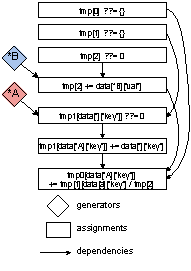
\includegraphics{images/intro_ir.pdf}
\end{minipage}
\begin{minipage}{0.62\textwidth}
\begin{lstlisting}[style=JavaScript,columns=flexible]
let tmp = {}
tmp[0] ??= {}
tmp[1] ??= {}                   
tmp[2] ??= 0                        
// sub-query de-correlated (loop hoisted)
(*@\highlight[highlightred]{for (let b in data)}@*) {
  tmp[2] += data[b]["val"]      // computes full aggregate
}
(*@\highlight[highlightblue]{for (let a in data)}@*) {
  tmp[1][data[a]["key"]] ??= 0
  tmp[1][data[a]["key"]] +=
            data[a]["key"]      // computes partial aggregate
  tmp[0][data[a]["key"]] = 
            tmp[1][data[a]["key"]] / tmp[2] // proportion

}
\end{lstlisting}
\end{minipage}
\caption{
On the left is the generated IR for the query in (a), comprising generators
(diamonds) representing iterators and assignments (rectangles) corresponding
to computations.
On the right is the JS code generated from this IR.
Notably, the `inner query' is hoisted in the final
generated code.
}\label{fig:ir_code}
\end{subfigure}

\caption{
The end-to-end workflow of \lang{}, starting with the query (a),
followed by the construction of the IR on the left side of (b), and the
final generated code on the right side of (b).
}\label{fig:intro}
\vspace{-5mm}
\end{figure}


In \Cref{fig:intro}, we show a glimpse of how our query language works end-to-end.
Note that our current implementation is done in JavaScript (JS) and we generate JS code for given input queries.
As shown in \Cref{fig:intro_query}, the dataset for this example consists of a collection
of objects, each featuring a \inline{key} and a \inline{val}.
The provided query computes the proportion of the sum of values corresponding to
each unique key with respect to the total sum of values.
We will formally introduce the syntax of the query language in \Cref{sec:query_language},
but, the general idea here is that \inline{*A} and \inline{*B} are iterators, and 
\inline{sum(data.*A.val)} nested inside \inline{data.*A.key} signifies the grouping of objects by the
\inline{key} and the subsequent computation of partial aggregates within these groups.
Conversely, since \inline{sum(data.*B.val)} is not nested within another \inline{*B}, it indicates
a complete aggregate computation (i.e., total sum of values).

\Cref{fig:ir_code} shows how the IR for the  for the aforementioned query is
constructed, along with a depiction of the final JS code generated from this IR.
The IR primarily comprises two fundamental components.
First, it contains generators, which represent the iterators essential for iterating
through a list of objects.
Second, it features assignments, which embody the computations necessary for executing
the query.
\inline{tmp[0]}, \inline{tmp[1]} and \inline{tmp[2]} corresponds to intermediate values
that are computed during the evaluation of the query.
Notably, the IR operates without explicit control flow constructs; instead, the
program's structure is implicit, established via dependencies.
These dependencies enables our compiler to perform optimizations like lambda lifting,
that would translate to sub-query hoisting that typically happens at logical plan level.
For instance, the expression \inline{sum(data.*B.val)} represents a nested sub-query,
which our compiler efficiently hoists as a separate loop in the generated code.
We will delve deep into each of these aspects of \lang{} in later sections of the paper.

The previous example exemplified \lang{}'s capability to express analytical queries on JSON
objects.
Nevertheless, the versatility of \lang{} extends far beyond this, encompassing an even broader
spectrum of use cases. 
For example, this includes its ability to articulate the visual aspects of web application
front-ends and its capacity to express tensor computations in a fashion reminiscent of
Einstein notation, among others.
\todo{point to the section of the paper}

% Throughout the paper we demonstrate \lang{}'s expressivity in a wide variety of
% use cases including, data querying (computing aggregates, joins, etc.), expressing
% visual aspects of web application front-ends, and also expressing tensor computations
% in a style similar to Einstein notation.


% TODO: maybe highlight the fact that this compositionality, mixing of visual aspects, etc.
%       is enabled by the fact that our query language resembles JSON so that we can directly
%       process that in JS

Our specific contributions are as follows.

\begin{itemize}
    \item We present the syntax of our query language and demonstrate how to express common
          data manipulation operators like, selections, group-bys, joins, user-defined functions (UDFs),
          and so on.
          Moreover, we show how to express visual components, and how to compose them to build
          large queries (\Cref{sec:query_language}).
    \item We show how the queries are lowered into an IR that contains loop-free and branch-free code
          with dependencies implicitly representing the program structure.
          Then, we demonstrate how this IR can be used to generate code for a given query by constructing
          the program structure from dependencies.
          Moreover, we show how traditional compiler optimizations like lambda lifting translates to query
          optimizations like sub-query de-correlation (\Cref{sec:ir_codegen}).
    \item We demonstrate the capabilities of our overall query language by taking a relatively simple example
          program that uses most of the features we have presented in previous sections (\Cref{sec:case_study}).
    \item We compare the performance of \lang{} on several practical JSON analytics workloads to demonstrate the
          effectiveness of our code generation approach (\Cref{sec:experiments}).
\end{itemize}

We discuss related work in \Cref{sec:related_work}, followed by conclusions and potential future research directions
in \Cref{sec:conclusions}.


\section{The Query Language}~\label{sec:query_language}

In the previous section, we saw \lang{} in action for a simple query.
In this section, we will formally introduce the syntax of the \lang{}, illustrating how it facilitates
the expression of common data manipulation operations like selections, aggregates,
group-bys, and so on.
To enhance comprehension, we will employ a running illustrative example dataset, as
depicted below.
Specifically, we have a dataset of containing population of several major cities,
along with the respective country.
Our chosen dataset is deliberately kept relatively straightforward, devoid of
intricate nested structures.
However, it is worth noting that \lang{} has the capacity to seamlessly query
deeply nested JSON data without any problem in the same way.


\begin{lstlisting}[style=JavaScript]
let data = [
    {country: "Japan", city: "Tokyo",     population: 14},
    {country: "China", city: "Beijing",   population: 22},
    {country: "France",city: "Paris",     population: 3},
    {country: "UK",    city: "London",    population: 9},
    {country: "Japan", city: "Osaka",     population: 3},
    {country: "UK",    city: "Birmingham",population: 2}
]
\end{lstlisting}

% \begin{lstlisting}[style=JavaScript]
% let data = [
%     {key: "A", val: 20},
%     {key: "B", val: 30},
%     {key: "A", val: 10}
% ]
% \end{lstlisting}

\subsection{Basics}
First we will look at how to perform several basic query operations on the
aforementioned dataset.
For instance, if we want to select a particular key of the dataset at a given
index, we can use the following syntax.

\begin{lstlisting}[style=JavaScript]
data.0.country              // result: Japan
{first : data.0.country}    // result: {first: Japan}
\end{lstlisting}

Several key attributes of \lang{} can be observed from the aforementioned examples.
In the given illustration, the reference \inline{data} refers to
the dataset object, enabling simple indexing into the array of data through integer
indices.
Furthermore, the selection of specific keys is facilitated by specifying the desired
key names (e.g., \inline{.country}).
Notably, \lang{} offers the convenience of the familiar JS-like syntax for constructing
structured output from extracted values, as exemplified in the second instance.

While this form of explicit indexing into the array can be useful for several
use cases, generally, queries involve some form of iterating over the dataset.
\lang{} offers this capability through the \inline{*} operator,
serving as an implicit iteration operator.
Later in our discussion, we will delve into how this operator empowers fine-grained
iterations, utilizing multiple iterators
(e.g., \inline{*A}, \inline{*B}, etc.).
For now, our focus centers on relatively simple queries.
Below, we present three example queries that leverage iterators and compute
aggregates over the iterated values.

\begin{lstlisting}[style=JavaScript, columns=flexible]
[data.*.city]             // result: [Tokyo, Beijing, ..., Birmingham]
sum(data.*.population)    // result: 53
max(data.*.population)    // result: 22
\end{lstlisting}

The queries presented above are self-explanatory in nature.
In the first example, we illustrate a scenario where an array can be constructed
from the values obtained through iteration, employing the \inline{[...]} syntax.
Alternatively, users can compute aggregates over the iterated values using the
relevant aggregate functions, such as \inline{sum}, \inline{max}, and so forth.
As discussed previously, this queries can be used as parts of object
construction logic and combined flexibly as shown below.

\begin{lstlisting}[style=JavaScript, columns=flexible, numbers=none]
    { total: sum(data.*.population), maximum: max(data.*.population) }
    // result: {total: 53, max: 22}
    \end{lstlisting}

% \begin{minipage}{0.5\textwidth}
% \begin{lstlisting}[style=JavaScript, columns=flexible, numbers=none]
% { 
%     total: sum(data.*.population),
%     maximum: max(data.*.population) 
% }
% \end{lstlisting}
% \end{minipage}

% \begin{minipage}{0.5\textwidth}
% \begin{lstlisting}[style=JSComment, columns=flexible, numbers=none]
% result: 
% {
%     total: 53,
%     max: 22
% }
% \end{lstlisting}
% \end{minipage}


\subsection{Group By}
Up to this point, we have explored fundamental query operations, including indexing,
iteration, and aggregate computation.
Another vital query operator, especially relevant to JSON-style objects,
is the group-by query.
\lang{} offers an intuitive means of implicitly expressing group-bys.
The following query exemplifies this, grouping records based on the
\inline{country} attribute and subsequently calculating the total population
for each group:

\begin{lstlisting}[style=JavaScript, columns=flexible, numbers=none]
{ data.*.country: sum(data.*.population) }
// result: {Japan: 17, China: 22, France: 3, UK: 11}
\end{lstlisting}

In the above syntax, specifying \inline{data.*.country} as the key implies
that any iteration carried out within this key utilizing the same
iterator (\inline{*}) is performed for records with each unique value of \inline{country}
separately.

The next example shown below demonstrates the versatility of \lang{} group-by queries, showcasing
aggregations at different levels.
Moreover, it underscores the composability of \lang{} queries.
This query computes the total population of all records, breaks it down by country,
and subsequently computes the population proportion of each city with respect to its
corresponding country:

\begin{lstlisting}[style=JavaScript, columns=flexible, numbers=none]
let countryPop = {data.*A.country: sum(data.*A.population)} // country -> total population
let query = { 
    total: sum(data.*.population),                                // total population
    data.*.country:
    {   total: get(countryPop, data.*.country)                    // total population per country
        data.*.city: div(sum(data.*.population),                  // population proportion
                            get(countryPop, data.*.country))} // (per each city)
}
// result: {total: 53. Japan: {total: 17, Tokyo: 0.82, Osaka: 0.18}, ...}
\end{lstlisting}

Specifically, the \inline{countryPop} is a separate query that determines the total
population for each country.
This query is subsequently utilized within the main \inline{query} to access the
total population for each country where required.



\subsection{Filters}
\todo{
    discuss about expressing filters. Duality with lambdas with if conditions.
}

\subsection{Join}
Joins are another fundamental operator in data querying.

Consider the following new dataset called \inline{other}.
This contains the \inline{region} that each country belongs to.
Now if want to compute aggregate population values over regions, we
have to join our original \inline{data} object with this new object
to obtain the corresponding region for each country.

\begin{lstlisting}[style=JavaScript]
let other = [
    {country: "Japan", region: "Asia"},
    {country: "China", region: "Asia"},
    {country: "France",region: "Europe"},
    {country: "UK",    region: "Europe"},
]
\end{lstlisting}

Shown below is how to express such a query in \lang{}.

\begin{lstlisting}[style=JavaScript, columns=flexible]
let countryToReg = {
    other.*O.country: other.*O.region
}
let query = {
    "-": merge(get(countryToReg, data.*.country), {
        data.*.city: sum("data.*.population")
    }),
}
\end{lstlisting}


\subsection{Used-defined Functions}
\subsection{Arrays}
\subsection{Fluent API}

\subsection{GUI Components}
Basic building blocks -- table definition, and generic display, svg, etc. 

\subsection{Tensor Expressions}
Matrix transpose, matrix multiplication and some other complex reduction?

\section{IR and Code Generation}~\label{sec:ir_codegen}
\subsection{IR Structure}
Loop-free and branch-free code, program structure implicit in dependencies

\subsection{Code Generation}
Scheduling based on dependencies, lambda lifting to de-correlate queries

\subsection{Incremental Execution}

\subsection{Implementation}
We implement this in JavaScript so that it can run in the browser.


\section{Example: Pivot Table}\label{sec:case_study}
How to use group bys, partial aggregates, display, svg, etc.

\section{Experiments}\label{sec:experiments}
We will have to variants: non-incremental and incremental.
For incremental we can show the execution time per each `batch' of
records (batch on x-axis).


\section{Related Work}\label{sec:related_work}
query languages, incremental triggers, FORWARD-style works that has the promise
of program = query.


\section{Conclusions and Future Work}\label{sec:conclusions}
Incrementality, Datalog-style recursive queries?, partial re-evaluation as
query changes (with minimal recomputation and index sharing)
%
% ---- Bibliography ----
%
% BibTeX users should specify bibliography style 'splncs04'.
% References will then be sorted and formatted in the correct style.

\bibliographystyle{splncs04}
\bibliography{references}
\end{document}
